\section{SSSP mit negativen Kanten}
\begin{frame}{Übersicht}
\begin{figure}[htbp]
\centering
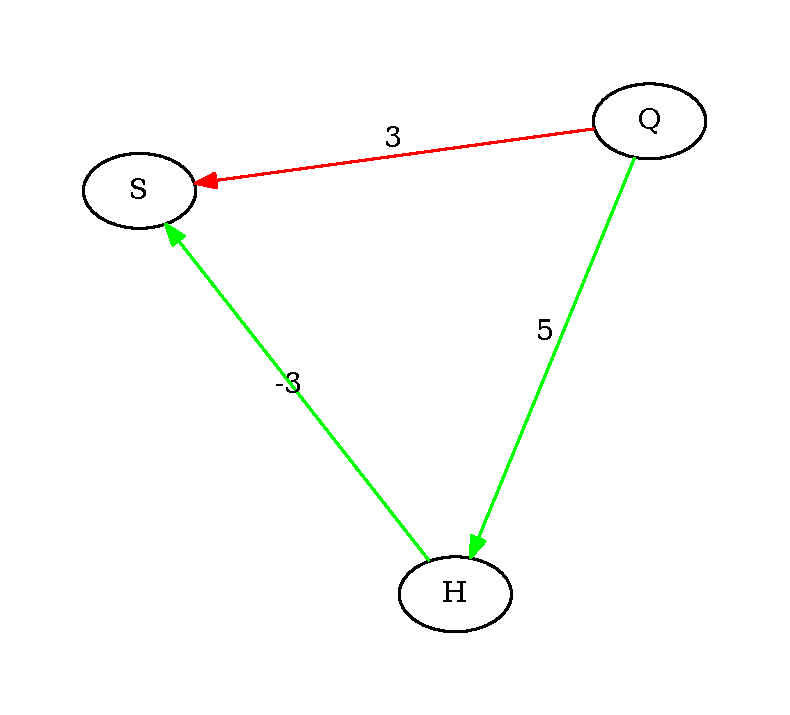
\includegraphics[width=\linewidth]{dijkstra_gegenbeispiel.pdf}
\end{figure}
\begin{alertblock}{Problem}
Dijkstra kommt nicht mit negativen Kanten zurecht
\end{alertblock}
\end{frame}

\begin{frame}{Ansätze}
\begin{itemize}
\item
  Lösung: rohe %\sout{Gewalt}
  Rechenleistung
\item
  Wichtige Einschränkung: negative Kreise auf irgendeinem Pfad von
  \texttt{Q} zu \texttt{S} bedeuten Nichtexistenz eines kürzesten Pfades
\item
  Idee 1: vollständige Tiefensuche.

  \begin{itemize}
  \item
    selbst für Brute-Force-Verhältnisse zu langsam (exponentielle
    Laufzeit)
  \end{itemize}
\end{itemize}
\end{frame}

\begin{frame}{Ansätze}
\begin{itemize}
\item
  Idee 2:
  \begin{itemize}
  \item
    kürzester Pfad enthält maximal $|V| - 1$ Kanten
  \item
    Enthalte der kürzeste Pfad $i$ Kanten. Falls wir alle kürzesten
    Pfade mit bis zu $i - 1$ Knoten kennen:

    \begin{itemize}
    \item
      Zu den kürzesten Pfaden mit bis zu $i$ Kanten fehlt höchstens eine
      Kante.
    \item
      Probiere für alle Kanten, ob sie irgendwo einen kürzeren Pfad
      erzeugen
    \end{itemize}
  \item
    Für $i = 0$ ist die Distanz der Quelle zu sich selbst 0, und die zu
    allen anderen Knoten $\inf$
  \end{itemize}
\item
  Idee 2 ist offensichtlich vielversprechender, sie führt zum
  Algorithmus von Bellman und Ford.
\end{itemize}
\end{frame}

\begin{frame}{Initialisierung}
\begin{figure}[htbp]
\centering
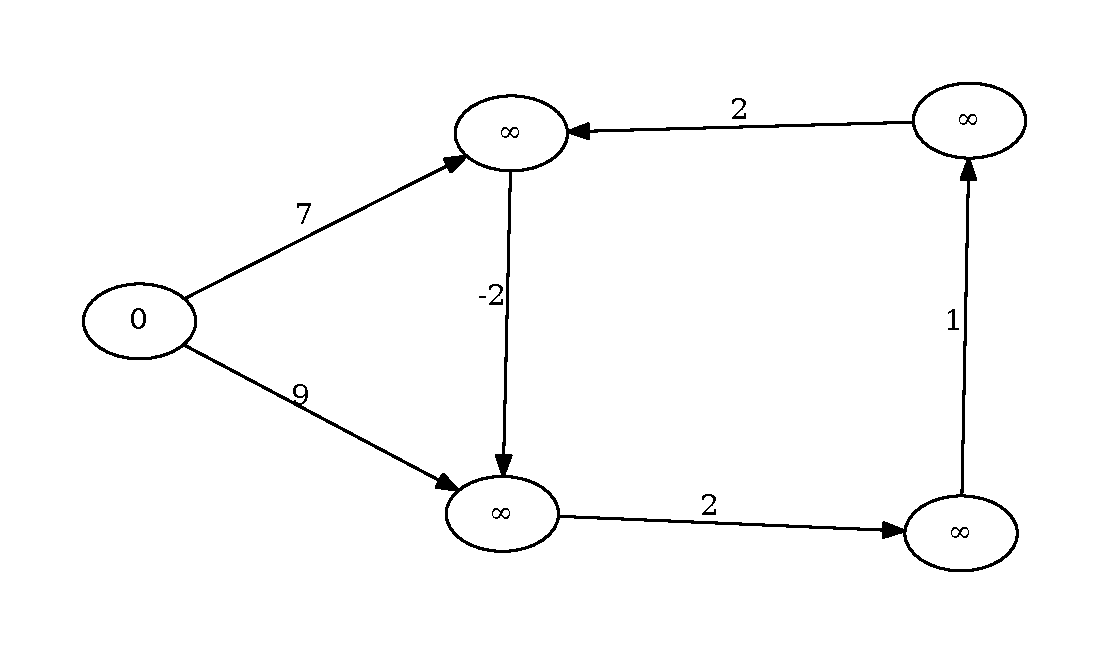
\includegraphics[width=\linewidth]{bellman_ford_graphs/graph_00.pdf}
\end{figure}
\end{frame}

\begin{frame}{Runde 1}
	\begin{block}{Runde 1}
	Relaxiere in \textit{beliebiger Reihenfolge} jede Kante einmal.
	\end{block}
\end{frame}

\begin{frame}{Runde 1}
\begin{figure}[htbp]
\centering
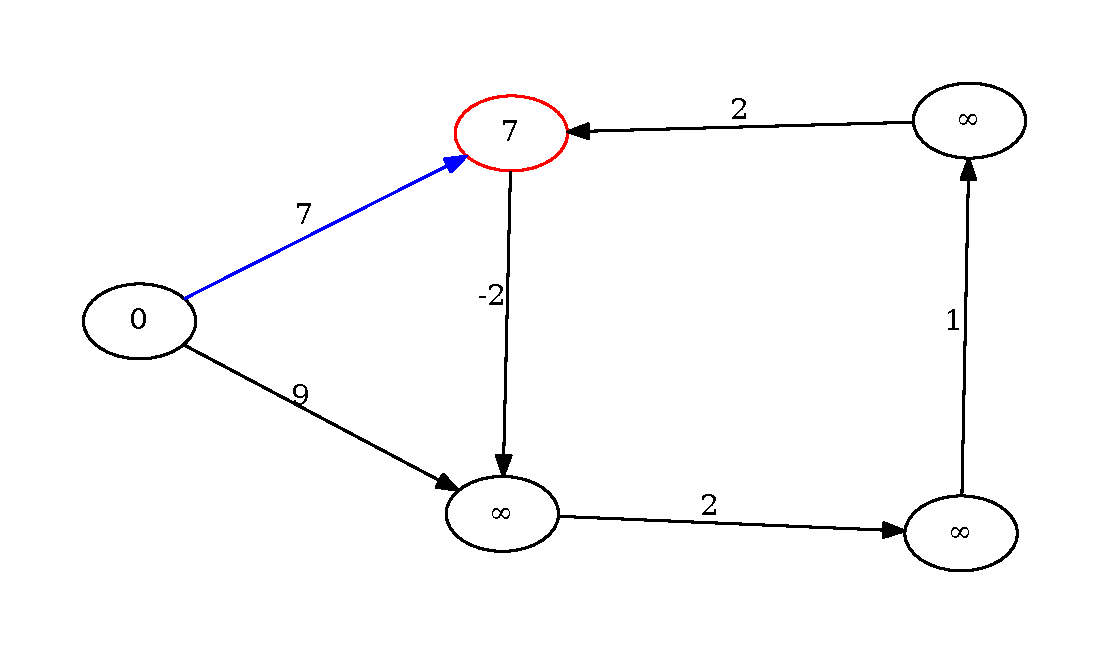
\includegraphics[width=\linewidth]{bellman_ford_graphs/graph_01.pdf}
\end{figure}
\end{frame}
\begin{frame}{Runde 1}
\begin{figure}[htbp]
\centering
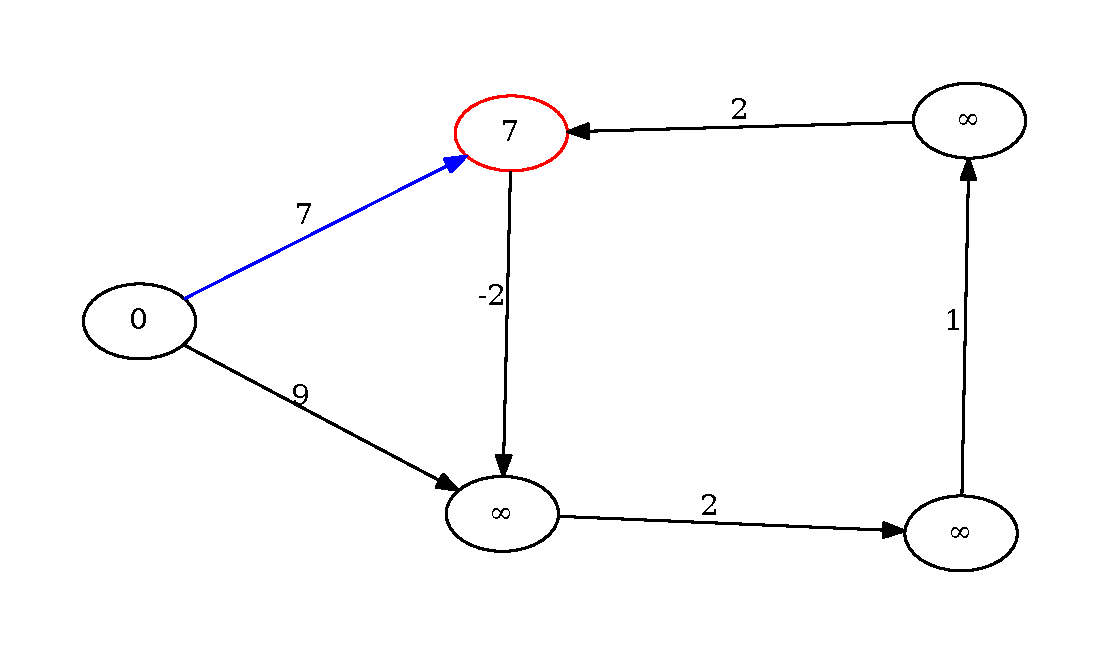
\includegraphics[width=\linewidth]{bellman_ford_graphs/graph_01.pdf}
\end{figure}
\end{frame}


\begin{frame}{Runde 1}
\begin{figure}[htbp]
\centering
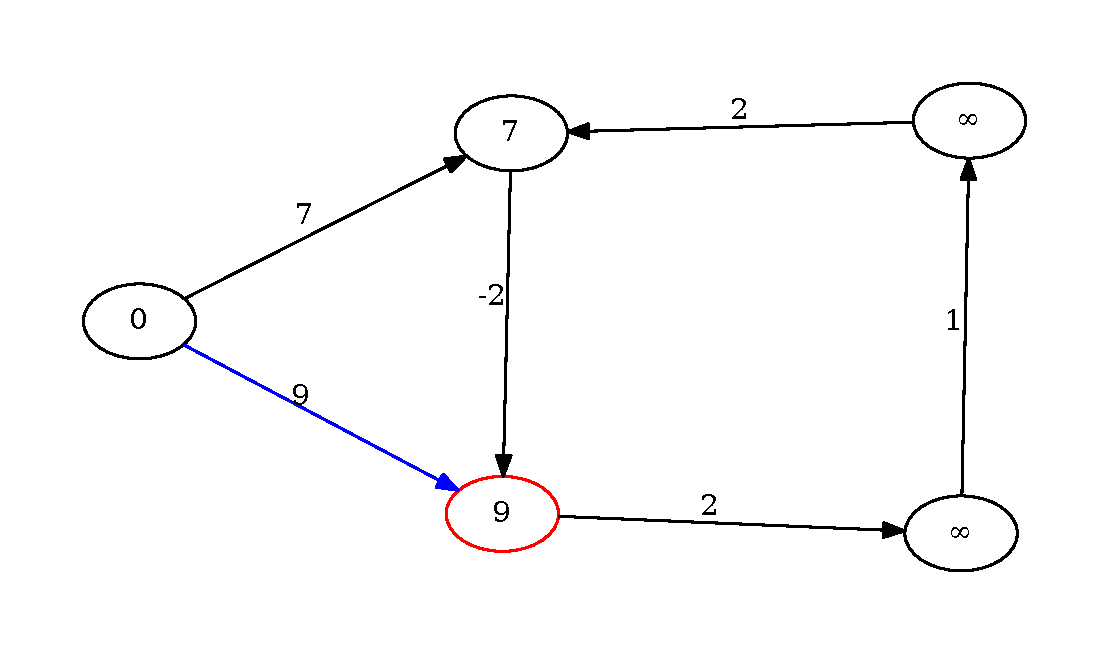
\includegraphics[width=\linewidth]{bellman_ford_graphs/graph_02.pdf}
\end{figure}
\end{frame}

\begin{frame}{Runde 1}
\begin{figure}[htbp]
\centering
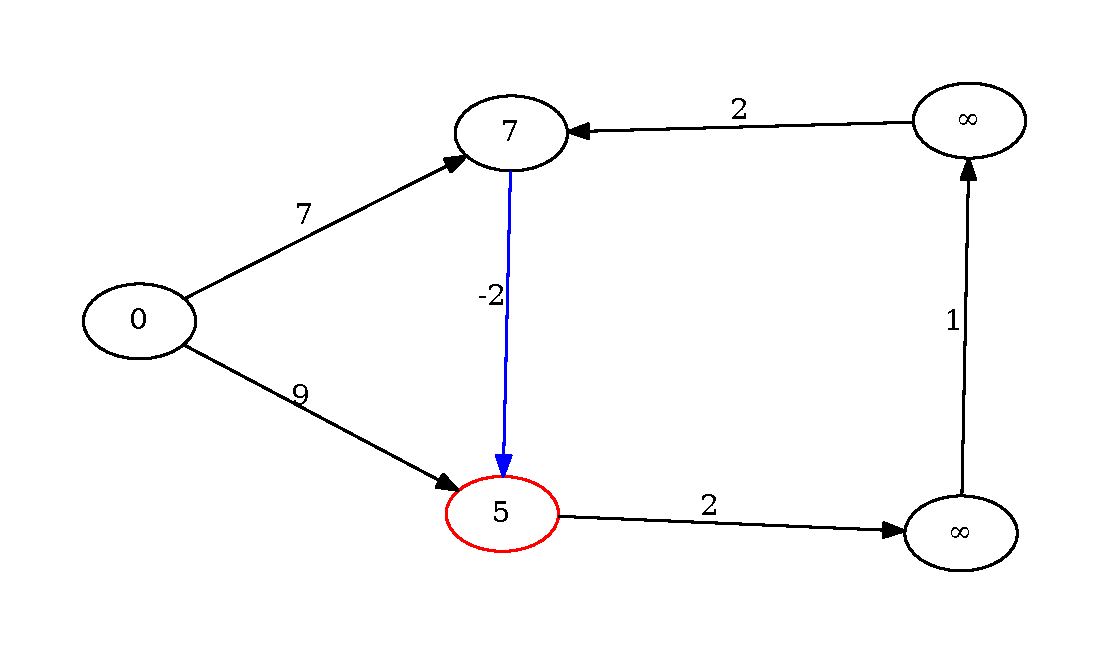
\includegraphics[width=\linewidth]{bellman_ford_graphs/graph_03.pdf}
\end{figure}
\end{frame}

\begin{frame}{Runde 1}
\begin{figure}[htbp]
\centering
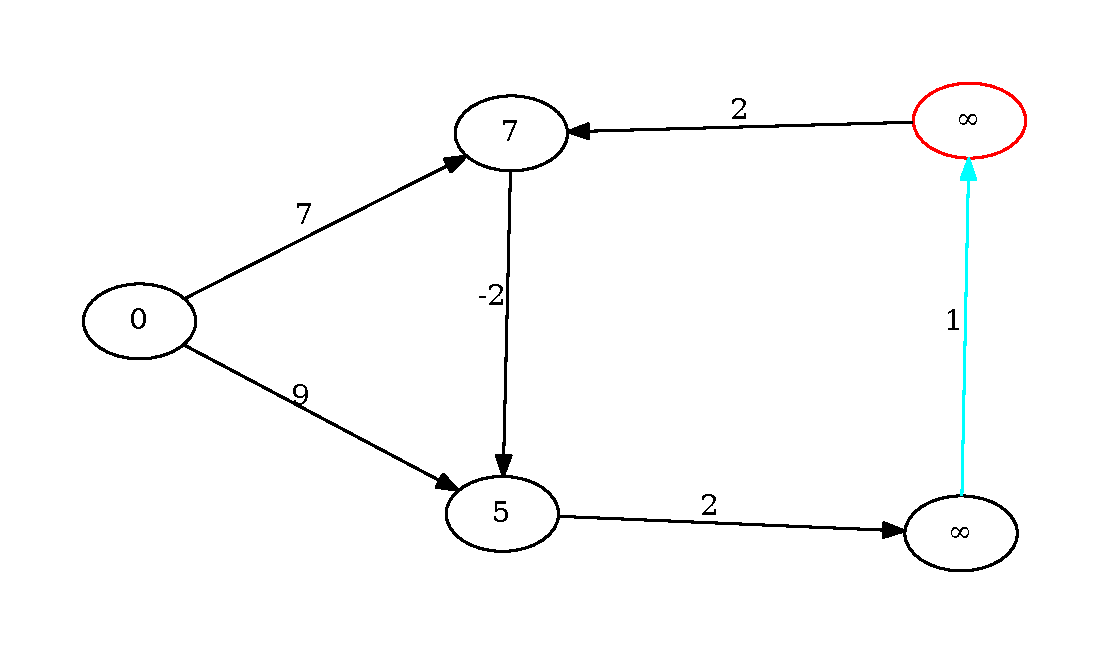
\includegraphics[width=\linewidth]{bellman_ford_graphs/graph_04.pdf}
\end{figure}
\end{frame}

\begin{frame}{Runde 1}
\begin{figure}[htbp]
\centering
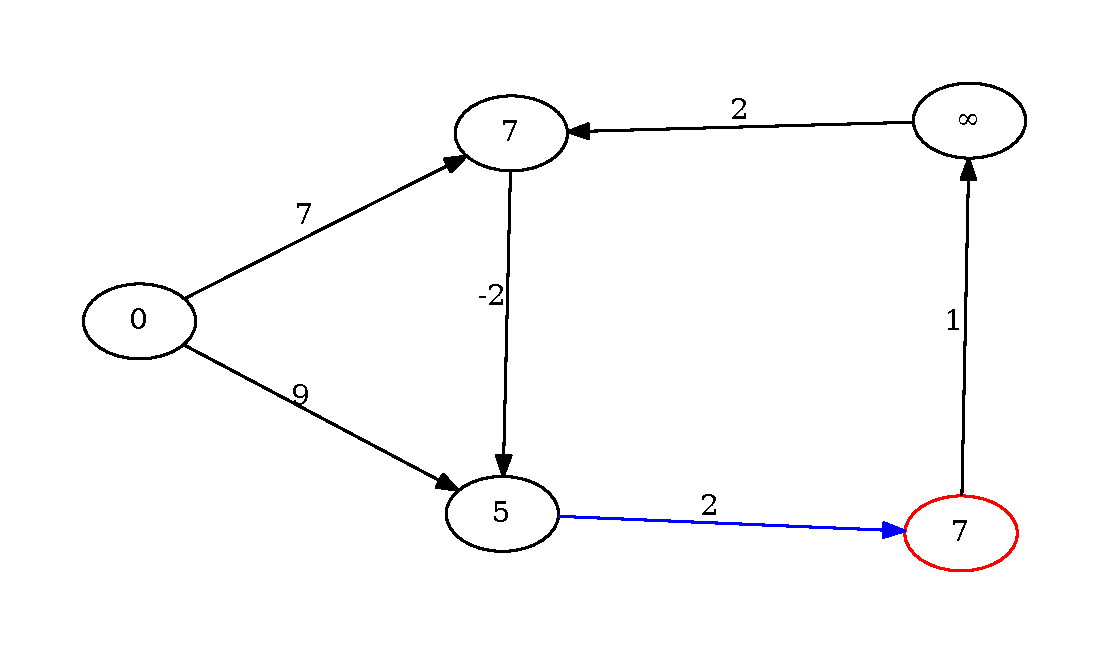
\includegraphics[width=\linewidth]{bellman_ford_graphs/graph_05.pdf}
\end{figure}
\end{frame}

\begin{frame}{Runde 1}
\begin{figure}[htbp]
\centering
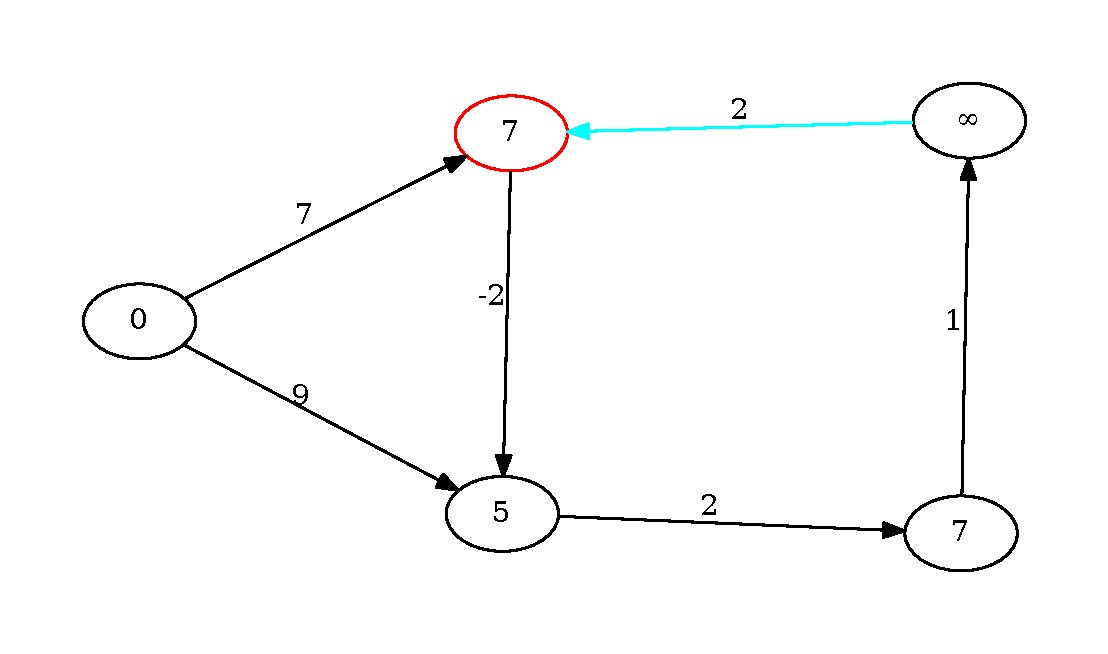
\includegraphics[width=\linewidth]{bellman_ford_graphs/graph_06.pdf}
\end{figure}
\end{frame}

\begin{frame}{Runde 2}
	\begin{block}{Runde 2}
	Wiederhole, da es Änderungen gab.
	\end{block}
\end{frame}

\begin{frame}{Runde 2}
\begin{figure}[htbp]
\centering
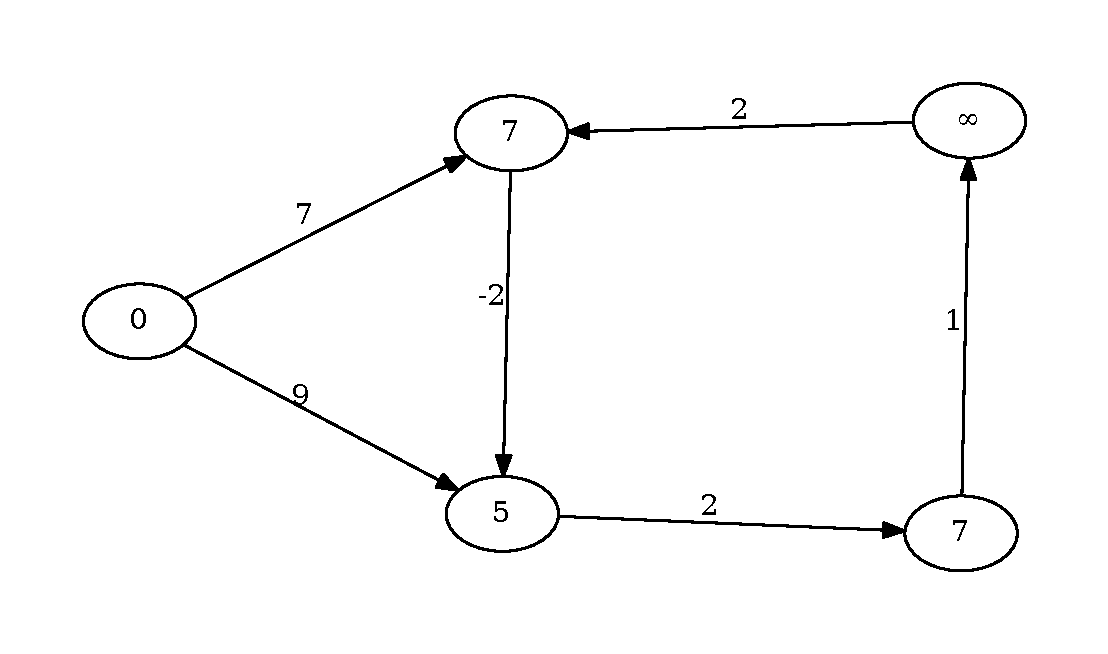
\includegraphics[width=\linewidth]{bellman_ford_graphs/graph_07.pdf}
\end{figure}
\end{frame}

\begin{frame}{Runde 2}
\begin{figure}[htbp]
\centering
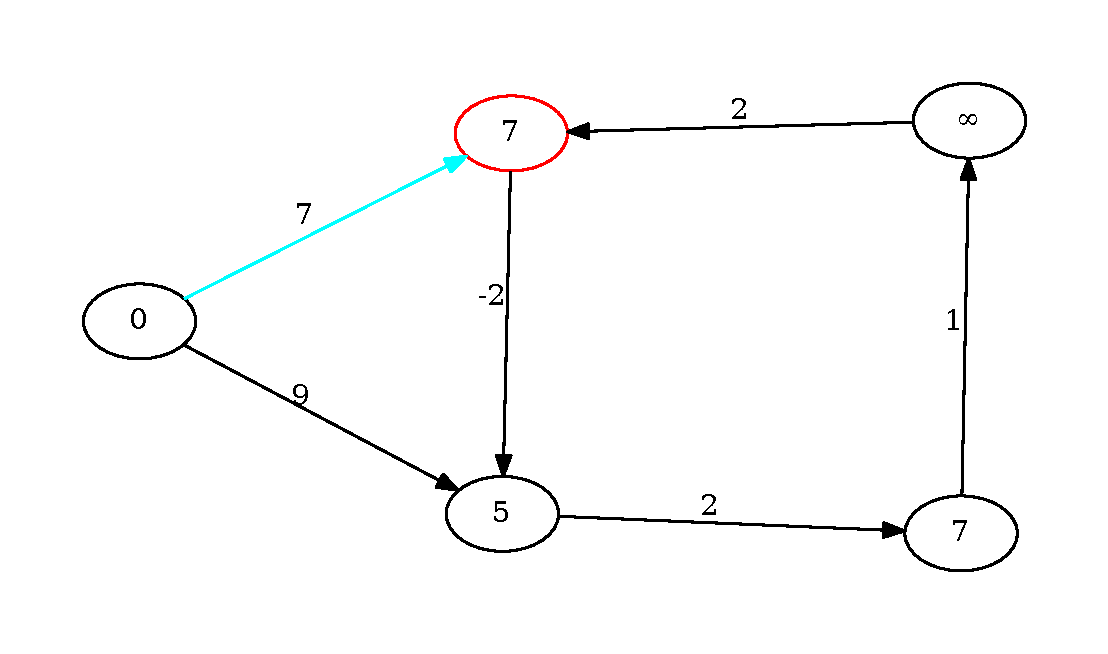
\includegraphics[width=\linewidth]{bellman_ford_graphs/graph_08.pdf}
\end{figure}
\end{frame}

\begin{frame}{Runde 2}
\begin{figure}[htbp]
\centering
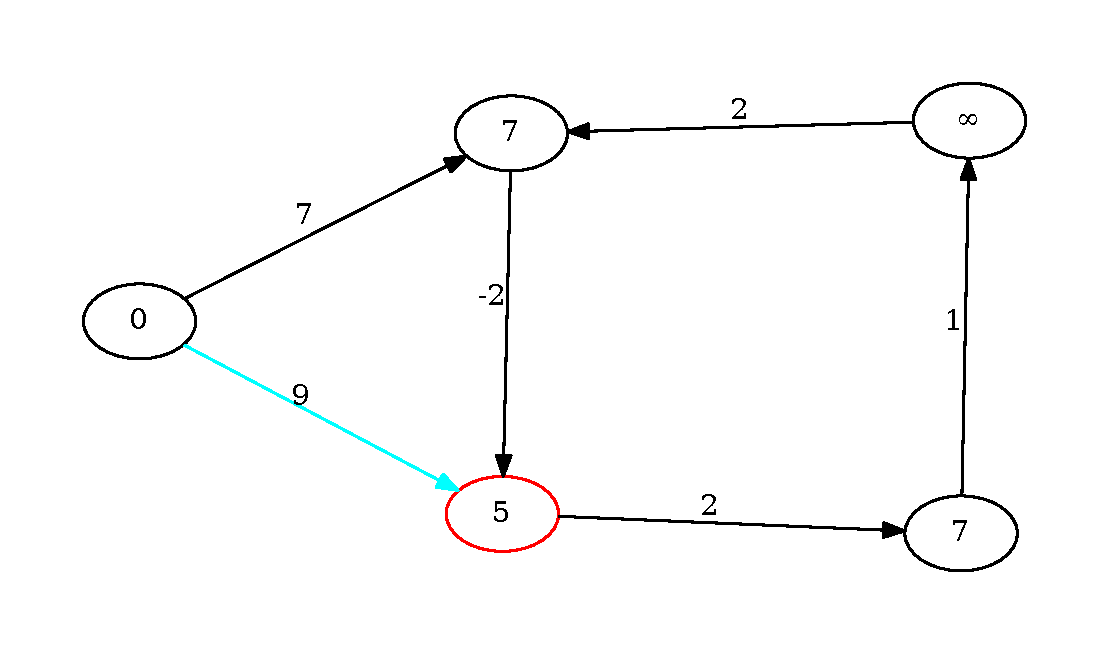
\includegraphics[width=\linewidth]{bellman_ford_graphs/graph_09.pdf}
\end{figure}
\end{frame}

\begin{frame}{Runde 2}
\begin{figure}[htbp]
\centering
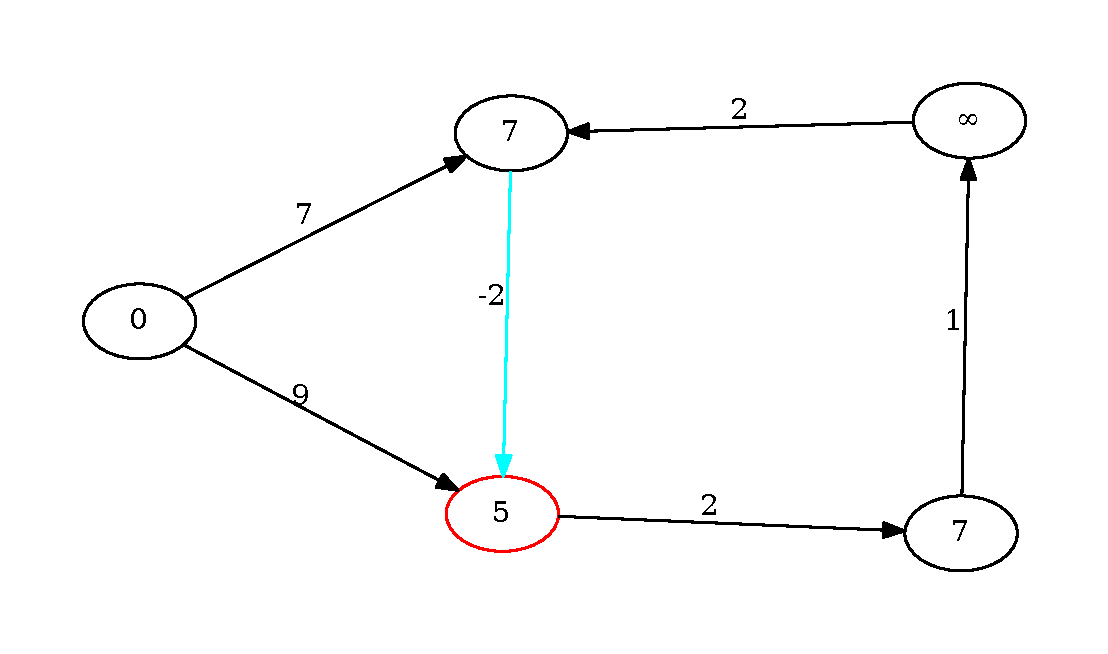
\includegraphics[width=\linewidth]{bellman_ford_graphs/graph_10.pdf}
\end{figure}
\end{frame}

\begin{frame}{Runde 2}
\begin{figure}[htbp]
\centering
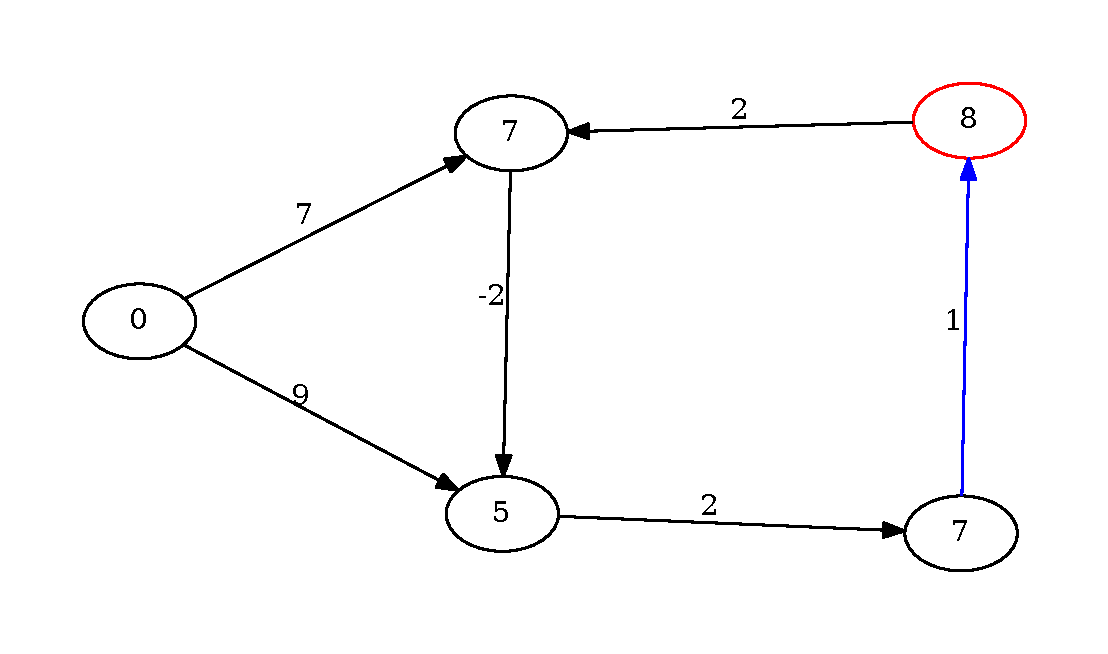
\includegraphics[width=\linewidth]{bellman_ford_graphs/graph_11.pdf}
\end{figure}
\end{frame}

\begin{frame}{Runde 2}
\begin{figure}[htbp]
\centering
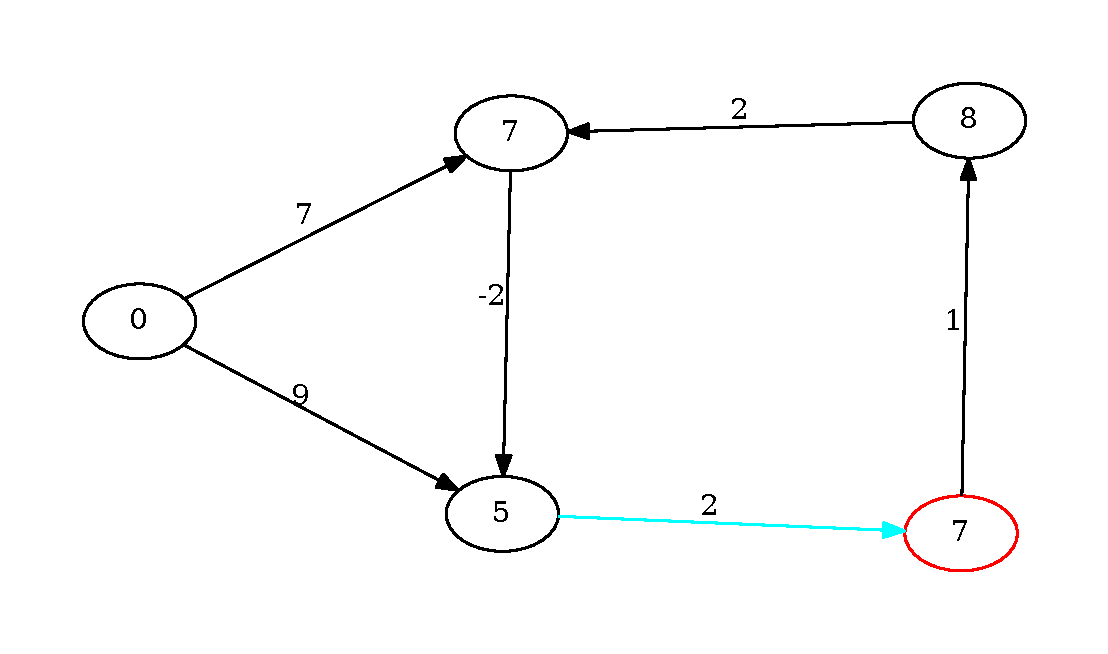
\includegraphics[width=\linewidth]{bellman_ford_graphs/graph_12.pdf}
\end{figure}
\end{frame}

\begin{frame}{Runde 2}
\begin{figure}[htbp]
\centering
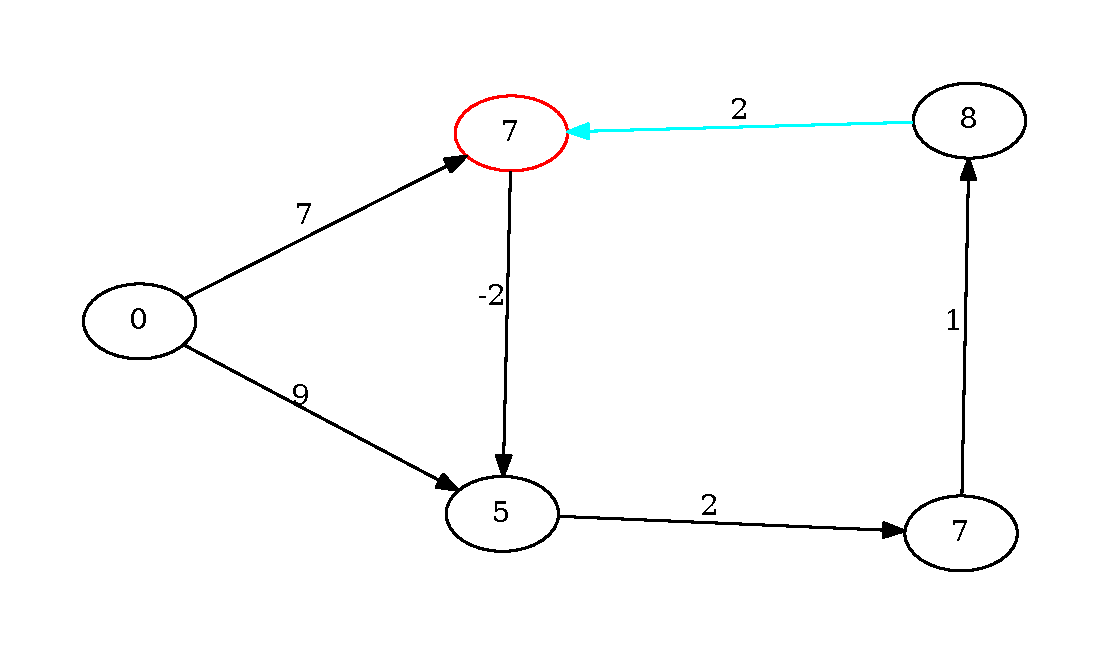
\includegraphics[width=\linewidth]{bellman_ford_graphs/graph_13.pdf}
\end{figure}
\end{frame}

\begin{frame}{Runde 3}
	\begin{block}{Runde 3}
	Wiederhole, da es Änderungen gab.
	\end{block}
	\begin{block}{Keine Änderungen}
	In der dritten Runde finden keine Relaxierungen mehr statt $\rightarrow$ fertig
	\end{block}
\end{frame}

\begin{frame}{Endergebnis}

\begin{figure}[htbp]
\centering
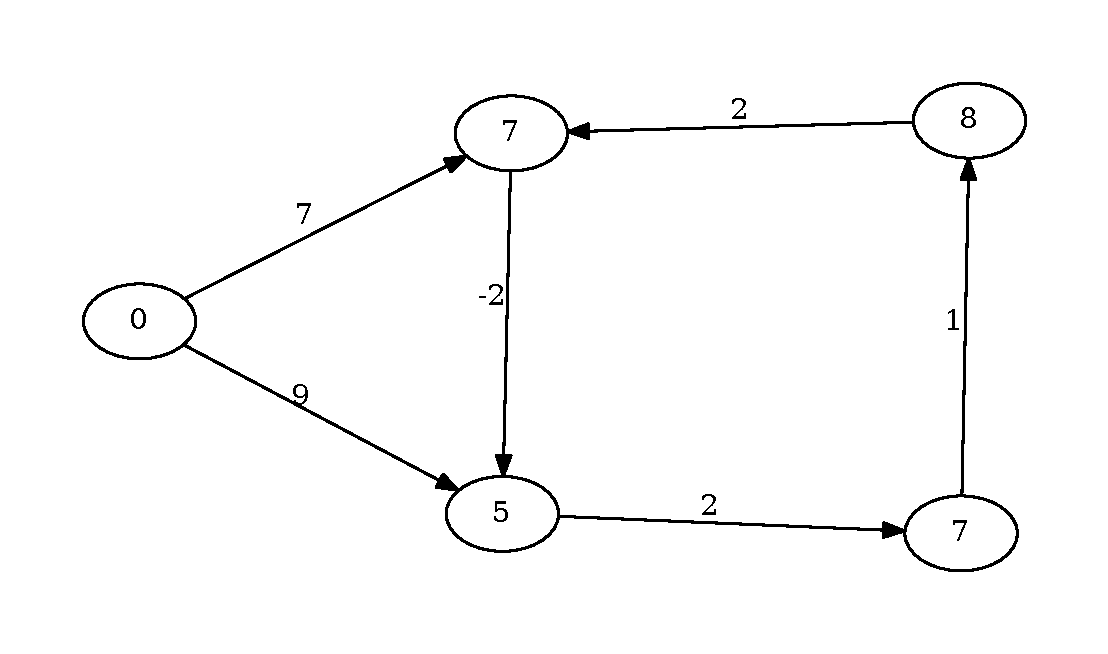
\includegraphics[width=\linewidth]{bellman_ford_graphs/graph_14.pdf}
\end{figure}

\end{frame}

\begin{frame}[fragile]{Code}
\begin{lstlisting}[basicstyle=\tiny]
using node = std::size_t;
const auto infinity = std::numeric_limits<double>::infinity();

struct edge {
    node from;
    node to;
    double dist;
};

std::vector<dist> bellman_ford(const std::size_t        node_count,
                               const std::vector<edge>& edges,
                               node                     source
) {
    std::vector<double> min_dists(node_count, infinity);
    min_dists[source] = 0;
    for (std::size_t i = 0; i < node_count + 1; ++i) {
        bool changes = false;
        for(const auto& e: edges) {
            const double old_dist = min_dists[e.to];
            const double new_dist = min_dists[e.from] + e.dist;
            if (new_dist < old_dist) {
                min_dists[e.to] = new_dist;
                changes = true;
            }
        }
        if (!changes) { break; }
        if (i == node_count) {
            throw std::runtime_error{"negative cycle"};
        }
    }
    return min_dists;
}
\end{lstlisting}
\end{frame}

\begin{frame}{Weitere Eigenschaften}
\begin{itemize}
	\item Negative Kreise lassen sich durch eine weitere Anwendung detektieren
	\item Die Entfernung von nicht über negative Kreise erreichbare Knoten wird immer korrekt ermittelt.
	\item In jedem negativen Kreis ändert sich im $n + 1$-ten Schritt mindestens eine Entfernung,
		die Detektion aller Knoten ohne Minimaldistanz ist somit leicht per Breitensuche möglich.
\end{itemize}
\end{frame}

\begin{frame}{Beurteilung}
\begin{itemize}
\itemsep1pt\parskip0pt\parsep0pt
\item
  Assymptotische Komplexität $\in O(n \cdot m)$
\item
  Profitiert nicht von kurzen Distanzen zwischen Quelle und Senke
\item
  Relativ leicht zu implementieren
\end{itemize}

\end{frame}

\begin{frame}{Fazit}

\begin{quote}
Kann man schon so machen, meistens will man das aber nicht
\end{quote}

\end{frame}
